% Este trabalho está licenciado sob a Licença Creative Commons Atribuição-CompartilhaIgual 3.0 Não Adaptada. Para ver uma cópia desta licença, visite http://creativecommons.org/licenses/by-sa/3.0/ ou envie uma carta para Creative Commons, PO Box 1866, Mountain View, CA 94042, USA.

\documentclass[../livro.tex]{subfiles}

\providecommand{\dir}{..}  %define o diretório principal

\begin{document}

\chapter{Semanas 14 e 15}

\section{Matrizes simétricas}

Uma \textbf{matriz simétrica} é uma matriz que é igual à sua transposta. Para que esta definição faça sentido, apenas podemos considerar matrizes que são quadradas. De forma mais precisa, se $A = \begin{bmatrix} a_{ij} \end{bmatrix}$ é uma matriz de orden $n \times n$, nós dizemos que $A$ é simétrica quando $A = A^T$.

Formas equivalentes de dizer que $A$ é simétrica incluem:
\begin{enumerate}[$(1)$]
	\item $A = A^T$;
	\item para todos os índices $i,j \in \{1,2,\dots,n\}$, temos que $a_{ij} = a_{ji}$;
	\item as colunas de $A$ são iguais às linhas de $A^T$;
	\item as linhas de $A$ são iguais às colunas de $A^T$.
\end{enumerate}

\begin{example}
	As matrizes
	\[
	\begin{bmatrix}
	1 & -3 \\
	-3 &  2
	\end{bmatrix}, \ \ 
	\begin{bmatrix}
	1 & -3 \\
	-3 &  1
	\end{bmatrix}, \ \ 
	\begin{bmatrix}
	1 & -3 & 0 \\
	-3 & -1 & 4 \\
	0 &  4 & 6
	\end{bmatrix} \checkmark
	\] são simétricas, enquanto  as matrizes
	\[
	\begin{bmatrix}
	1 & -3 \\
	3 &  1
	\end{bmatrix},\ \ 
	\begin{bmatrix}
	1 &  3 \\
	-3 &  2
	\end{bmatrix},\ \ 
	\begin{bmatrix}
	1 & -3 &  0 \\
	4 & -1 & -3 \\
	0 &  4 &  1
	\end{bmatrix} \textsc{x}
	\] não são. Deve-se tomar o cuidado de verificar a simetria \textit{com relação à diagonal principal}. Qualquer outro tipo de simetria não deve interferir na nossa análise$. \ \lhd$
\end{example}

Um dos resultados mais importantes de Álgebra Linear é o Teorema Espectral, que diz que toda matriz simétrica é diagonalizável por uma base de autovetores que é ortonormal. De forma mais precisa:

\begin{teoespectral}
	Suponhamos que $A$ é uma matriz simétrica com coeficientes reais. Então:
	\begin{enumerate}[$(i)$]
		\item todos os autovalores de $A$ são reais;
		\item autovetores associados a autovalores distintos são ortogonais.
		\item a dimensão do autoespaço associado a um autovalor é igual à multiplicidade deste autovalor como raiz do polinômio característico;
		\item existe uma base ortonormal de $\bR^n$ formada por autovetores de $A$;
		\item $A$ é diagonalizável por uma matriz de mudança de coordenadas ortonormal $P$: a matriz $P$ cujas colunas são os autovetores (ortonormais) de $A$ é tal que 
		\[
		P^{T} A P = P^{-1} A P = D.
		\]
	\end{enumerate}
\end{teoespectral}

Nós vamos apresentar uma prova deste resultado no final destas notas. Antes de mais nada, faremos alguns exemplos e aplicações que justificam a importância do Teorema Espectral. No entanto, é fortemente aconselhado que o leitor acompanhe os elementos da demonstração, para efetivamente entender as propriedades essenciais das matrizes simétricas.

\begin{example}
	Considere
	\[
	A = \begin{bmatrix}
	1 & -5 \\
	-5 &  1
	\end{bmatrix}.
	\] O polinômio característico é
	\[
	\det \begin{bmatrix}
	1-\lambda & -4 \\
	-4 & 5-\lambda
	\end{bmatrix} = (1-\lambda)^2 - 25 = \lambda^2 - 2 \lambda - 24
	\] cujas raízes são $6$ e  $-4$. Os autovetores são calculados como
	\[
	A + 4 I = 
	\begin{bmatrix}
	5 & -5 \\
	-5 & 5
	\end{bmatrix} \sim 
	\begin{bmatrix}
	1 & -1 \\
	0 & 0
	\end{bmatrix} \implies 
	\left\{
	\begin{array}{l}
	v_1 = v_2 \\ 
	\text{uma variável livre}
	\end{array}
	\right. \implies \vec{v}_1 = v_2
	\begin{bmatrix}
	1  \\
	1
	\end{bmatrix}.
	\] Associado com $6$:
	\[
	A - 6 I = 
	\begin{bmatrix}
	-5 & -5 \\
	-5 & -5
	\end{bmatrix} \sim 
	\begin{bmatrix}
	1 & 1 \\
	0 & 0
	\end{bmatrix} \implies 
	\left\{
	\begin{array}{l}
	v_2 = - v_1 \\ 
	\text{uma variável livre}
	\end{array}
	\right. \implies \vec{v}_2 = v_2
	\begin{bmatrix}
	1 \\
	-1
	\end{bmatrix}.
	\] Uma base de autovetores é
	\[
	\left\lbrace 
	\begin{bmatrix}
	1 \\
	1
	\end{bmatrix}, 
	\begin{bmatrix}
	1 \\
	-1
	\end{bmatrix}
	\right\rbrace.
	\] Observe que são de fato reais os autovalores e que os autovetores associados são ortogonais (faça a conta!). Se quisermos uma base ortonormal para $\bR^2$ formada por autovetores, normalizamos os que já obtivemos:
	\[
	\bR^2 = \Span \left\lbrace 
	\begin{bmatrix}
	1/\sqrt{2} \\
	1/\sqrt{2}
	\end{bmatrix}, 
	\begin{bmatrix}
	1/\sqrt{2} \\
	-1/\sqrt{2}
	\end{bmatrix}
	\right\rbrace.
	\] Lembrando do nosso processo de diagonalização, sabemos que
	\[
	P =  
	\begin{bmatrix}
	1/\sqrt{2} &  1/\sqrt{2} \\
	1/\sqrt{2} & -1/\sqrt{2} 
	\end{bmatrix} \implies 
	P^{-1} A P = 
	\begin{bmatrix}
	1/\sqrt{2} &  1/\sqrt{2} \\
	1/\sqrt{2} & -1/\sqrt{2} 
	\end{bmatrix}
	\begin{bmatrix}
	1 & -5 \\
	-5 &  1
	\end{bmatrix}
	\begin{bmatrix}
	1/\sqrt{2} &  1/\sqrt{2} \\
	1/\sqrt{2} & -1/\sqrt{2} 
	\end{bmatrix} = 
	\begin{bmatrix}
	-4 & 0 \\
	0  & 6
	\end{bmatrix}.
	\] A matriz $P$ que montamos acima é uma matriz ortogonal (de modo que $P^{-1} = P^T$), pois sabemos que autovetores associados com autovalores distintos são ortogonais e fizemos a normalização dos autovetores (lembra que uma matriz ortogonal deve ter colunas ortonormais)$. \ \lhd$
\end{example}


\begin{example}
	Vamos aplicar o procedimento de diagonalização para encontrar uma base ortonormal de autovetores de uma matriz de ordem $3 \times 3$. Considere a matriz simétrica
	\[
	A = 
	\begin{bmatrix}
	3 & -2 & 4 \\  
	-2 & 6 & 2 \\
	4 & 2 & 3 \\
	\end{bmatrix}.
	\] O polinômio característico de $A$ é 
          \begin{align*}
	p(\lambda) = \det (A - \lambda I ) & = 
	\det 
	\begin{bmatrix}
	3- \lambda & -2 & 4 \\  
	-2 & 6- \lambda & 2 \\
	4 & 2 & 3- \lambda \\
	\end{bmatrix} \\
	& = (3-\lambda) \left[ (6 - \lambda)(3 - \lambda) - 4 \right] + 2 \left[ -6 + 2 \lambda - 8 \right]  + 4 \left[ - 4 - 24 + 4 \lambda \right]  \\
	& = (3-\lambda) \left[ \lambda^2 - 9 \lambda + 14 \right] -28 + 4 \lambda - 112 + 16 \lambda  \\
	& = 3\lambda^2 - 27 \lambda + 42  - \left[ \lambda^3 - 9 \lambda^2 + 14 \lambda \right] + 20 \lambda - 140  \\
	& = -\lambda^3 + 12 \lambda^2 - 21 \lambda - 98.
          \end{align*}
 Como sabemos, se os coeficientes da matriz simétrica acima fossem escolhidos de maneira aleatória, dificilmente conseguiríamos encontrar as raízes deste polinômio com precisão. De qualquer forma, quaisquer raízes racionais (este exemplo foi construido artificialmente) deste polinômio só podem ser divisores de $98$ dividido pelos divisores de $-1$, isto é: $\pm 1, \pm 2, \pm 7, \pm 14, \pm 21$. Testando os primeiros, vemos que $-2$ é uma raiz. Pela divisão de polinômios, fatoramos
	\[
	p(\lambda) = -(\lambda + 2) (\lambda^2 - 14 \lambda + 49) = -(\lambda + 2)(\lambda - 7)^2.
	\] Logo, os autovalores de $A$ são $-2$ (simples) e $7$ (duplo).
	\begin{itemize}
		\item Autoespaço associado com o autovalor $-2$:
		\[
		A + 2 I = 
		\begin{bmatrix}
		5 & -2 & 4 \\  
		-2 & 8 & 2 \\
		4 & 2 & 5 \\
		\end{bmatrix} \sim
		\begin{bmatrix}
		-1 & 4 & 1 \\
		5 & -2 & 4 \\  
		4 & 2 & 5 \\
		\end{bmatrix} \sim 
		\begin{bmatrix}
		-1 & 4 & 1 \\
		0 & 18 & 9 \\  
		0 & 18 & 9 \\
		\end{bmatrix} \sim
		\begin{bmatrix}
		-1 & 2 & 0 \\
		0 &  2 & 1 \\  
		0 &  0 & 0 \\
		\end{bmatrix} \leftrightsquigarrow
		\left\lbrace 
		\begin{array}{l}
		v_1 = 2 v_2 \\
		v_3 = - 2 v_2 \\
		\text{1 variável livre}
		\end{array}
		\right. 
		\] Assim, um autovetor associado é ($v_2 = 1$)
		\[
		\vec{v}_1 = 
		\begin{bmatrix}
		2 \\ 1 \\ -2
		\end{bmatrix}.
		\]
		\item Autoespaço associado com o autovalor $7$:
		\[
		A - 7 I = 
		\begin{bmatrix}
		-4 & -2 & 4 \\  
		-2 & -1 & 2 \\
		4 & 2 & -4 \\
		\end{bmatrix} \sim
		\begin{bmatrix}
		-2 & -1 & 2 \\
		2 & 1 & -2 \\  
		0 & 0 & 0 \\
		\end{bmatrix} \sim 
		\begin{bmatrix}
		-2 & -1 & 2 \\
		0 & 0 & 0 \\  
		0 & 0 & 0 \\
		\end{bmatrix} \leftrightsquigarrow
		\left\lbrace 
		\begin{array}{l}
		v_2 = - 2 v_1 + 2 v_3  \\
		\text{2 variáveis livres}
		\end{array}
		\right. 
		\] Assim, qualquer autovetor pode ser escrito parametricamente como
		\[
		\vec{v} = 
		\begin{bmatrix}
		v_1 \\
		- 2 v_1 + 2v_3 \\
		v_3
		\end{bmatrix} = v_1 
		\begin{bmatrix}
		1 \\ -2 \\ 0
		\end{bmatrix} + v_2
		\begin{bmatrix}
		0 \\ 2 \\ 1
		\end{bmatrix}.
		\] Já era de se esperar que encontraríamos duas variáveis livres, porque sabemos (item $(iii)$ do Teorema Espectral) que deve ser dois a dimensão do autoespaço associado com um autovalor de multiplicidade dois.\footnote{Enfatizamos que isto não é verdade para qualquer matriz, apenas para as simétricas!} Concluimos que uma base para o autoespaço $\Nul (A - 7I)$ é
		\[
		\left\lbrace
		\vec{v}_2 = \begin{bmatrix}
		1 \\ -2 \\ 0
		\end{bmatrix}, \vec{v}_3 = 
		\begin{bmatrix}
		0 \\ 2 \\ 1
		\end{bmatrix}
		\right\rbrace.
		\]
	\end{itemize}
	
	Observamos que, em concordância com o item $(ii)$ do Teorema Espectral, autovetores associados a autovalores distintos são ortogonais: temos que $\vec{v}_1$ é ortogonal a cada um dos vetores $\vec{v}_2$ e $\vec{v}_3$ (faça as contas!). No entanto, estes três vetores não são ortogonais, pois os dois autovetores que estão associados com o mesmo autovalor satisfazem $\vec{v}_2 \cdot \vec{v}_3 = -4 \neq 0.$
	
	O fato de que os três autovetores que encontramos não são ortogonais não contradiz o Teorema Espectral. Pelo que vimos, o autoespaço associado com o autovalor $7$ tem dimensão dois. Encontramos uma base da maneira usual, mas ocorre que esta base não é ortogonal. Para obter uma base ortogonal, aplicamos o procedimento de Gram-Schmidt:
	\[
	\vec{u}_2 = \vec{v}_2 = 
	\begin{bmatrix}
	1 \\ -2 \\ 0
	\end{bmatrix}
	\]
	\[
	\vec{u}_3 = \vec{v}_3 - \proj_{\vec{u}_2} \vec{v}_3 = \vec{v}_3 - \frac{\vec{v}_3 \cdot \vec{u}_2}{\vec{u}_2 \cdot \vec{u}_2} \, \vec{u}_2 = 
	\begin{bmatrix}
	0 \\ 2 \\ 1
	\end{bmatrix} - \frac{-4}{5}
	\begin{bmatrix}
	1 \\ -2 \\ 0
	\end{bmatrix} = 
	\begin{bmatrix}
	4/5 \\ 2/5 \\ 1
	\end{bmatrix} \xrightarrow{\text{podemos considerar } \times 5}
	\begin{bmatrix}
	4 \\ 2 \\ 5
	\end{bmatrix}
	\] Agora
	\[
	\left\lbrace
	\begin{bmatrix}
	2 \\ 1 \\ -2
	\end{bmatrix}, \
	\begin{bmatrix}
	1 \\ -2 \\ 0
	\end{bmatrix}, \
	\begin{bmatrix}
	4 \\ 2 \\ 5
	\end{bmatrix}
	\right\rbrace.
	\] é uma base ortogonal de $\bR^3$ formada por autovalores da matriz $A$. Para obter uma base ortonormal, basta normalizar cada um dos vetores da base:
	\[
	\left\lbrace
	\begin{bmatrix}
	2/3 \\ 1/3 \\ -2/3
	\end{bmatrix}, \
	\begin{bmatrix}
	1/\sqrt{5} \\ -2/\sqrt{5} \\ 0
	\end{bmatrix}, \
	\begin{bmatrix}
	4/(3\sqrt{5}) \\ 2/(3\sqrt{5}) \\ 5/(3\sqrt{5})
	\end{bmatrix}
	\right\rbrace.
	\] Pelo método de diagonalização de matrizes, concluimos que $A$ pode ser diagonalizada pela matriz 
	\[
	P = 
	\begin{bmatrix}
	2/3  & 1/\sqrt{5}  & 4/(3\sqrt{5}) \\ 
	1/3  & -2/\sqrt{5} & 2/(3\sqrt{5}) \\ 
	-2/3 &       0     & 5/(3\sqrt{5})
	\end{bmatrix},
	\] que, neste caso (em que $A$ é matriz simétrica), pode ser obtida ortogonal. Sendo $P$ ortogonal, tem-se $P^{-1} = P^T$ e portanto $P^{T} A P =  D$, isto é,
	\[
	\begin{bmatrix}
	2/3  & 1/\sqrt{5}  & 4/(3\sqrt{5}) \\ 
	1/3  & -2/\sqrt{5} & 2/(3\sqrt{5}) \\ 
	-2/3 &       0     & 5/(3\sqrt{5})
	\end{bmatrix}
	\begin{bmatrix}
	5 & -2 & 4 \\  
	-2 & 8 & 2 \\
	4 & 2 & 5 \\
	\end{bmatrix}
	\begin{bmatrix}
	2/3  & 1/\sqrt{5}  & 4/(3\sqrt{5}) \\ 
	1/3  & -2/\sqrt{5} & 2/(3\sqrt{5}) \\ 
	-2/3 &       0     & 5/(3\sqrt{5})
	\end{bmatrix} = 
	\begin{bmatrix}
	-2& 0 & 0 \\
	0 & 7 & 0 \\
	0 & 0 & 7 \\
	\end{bmatrix}. \ \lhd
	\]
\end{example}


Enfatizamos ainda mais uma vez a aplicação do Teorema Espectral: ele afirma que, no caso de uma matriz simétrica $A$, o procedimento que aplicamos nos exemplos acima sempre vai funcionar! Teremos todos os autovalores reais. Sendo um autovalor $\lambda$ de multiplicidade $m$, seremos capazes de encontrar $m$ autovetores linearmente independentes, que geram o autoespaço $\Nul (A - \lambda I)$. Estes podem ser ortonormalizados pelo processo de Gram-Schmidt. Além disso, associados a autovalores distintos, temos autovetores ortogonais, de modo que seremos capazes de obter uma base ortonormal de autovetores de $A$.


\subsection{Formas quadráticas}


Nesta seção, apresentamos uma aplicação matemática de matrizes simétricas. Uma \textbf{forma quadrática} em $\bR^n$ é uma função polinomial em que todos os termos são de grau 2.

\begin{example}\label{exemplo1}
	A função $Q : \bR^2 \to \bR$, definida por 
	\[
	Q(x_1, x_2) = 3 x_1^2 + x_1x_2
	\] é uma forma quadrática em $\bR^2$, já que cada um dos termos tem grau 2.
	
	Mais geralmente, qualquer forma quadrática em $\bR^2$ pode ser escrita como
	\[
	Q(x_1, x_2) = a x_1^2 + 2 b x_1x_2 + cx_2^2,
	\] onde $a,b,c \in \bR$, já que os três termos acima são todos os possíveis monômios de grau dois em duas variáveis $x_1$ e $x_2$. O coeficiente $2$ que aparece no segundo termo é motivado pela fórmula mais geral (\ref{geral}) abaixo (observe que cada termo $x_i x_j$ aparece duas vezes na soma).
\end{example}




\begin{example}\label{exemplo2}
	A função $Q : \bR^3 \to \bR$, definida por 
	\[
	Q(x_1, x_2, x_3) = x_2^2 - x_3^2 + 3 x_1 x_2 - 8 x_1 x_3
	\] é uma forma quadrática em $\bR^3$. Qualquer forma quadrática em $\bR^3$ pode ser escrita como
	\[
	Q(x_1, x_2) = a x_1^2 + b x_2^2 + cx_3^2 + 2 dx_1x_2 +2  ex_1x_3 +2  fx_2x_3,
	\] onde $a,b,c, d, e, f \in \bR$.
\end{example}


De forma geral, uma forma quadrática $Q :\bR^n \to \bR$ pode ser escrita como
\begin{equation}\label{geral}
Q(x_1, x_2, \dots, x_n) = \sum_{i=1}^{n} \sum_{j=1}^{n} a_{ij} x_i x_j,
\end{equation} onde cada um dos coeficientes $a_{ij}$ são números reais. Podemos também supor que a matriz $A = (a_{ij})$ é simétrica.\footnote{Caso  $Q(x_1, x_2, \dots, x_n) = \sum_{i=1}^{n} \sum_{j=1}^{n} b_{ij} x_i x_j$ com uma matriz $B = (b_{ij})$  não  simétrica, podemos escrever $Q(x_1, x_2, \dots, x_n) = \sum_{i=1}^{n} b_{ii} x_i^2 + \sum_{i < j} (b_{ij} + b_{ji}) x_i x_j$. Definindo $a_{ij} = \frac{b_{ij} + b_{ji}}{2}$ temos também $Q(x_1, x_2, \dots, x_n) = \sum_{i=1}^{n} a_{ii} x_i^2 + 2 \sum_{i < j} a_{ij} x_i x_j$. Esta forma é mais semelhante com as dos exemplos acima. Note como aparece o coeficiente 2 nos termos com $i \neq j$. Finalmente, observamos que $A = (a_{ij})$ é uma matriz simétrica e que $\sum_{i=1}^{n} \sum_{j=1}^{n} b_{ij} x_i x_j = \sum_{i=1}^{n} a_{ii} x_i^2 + 2 \sum_{i < j} a_{ij} x_i x_j = \sum_{i=1}^{n} \sum_{j=1}^{n} a_{ij} x_i x_j.$}


Notamos o seguinte: se $A$ é uma matriz de ordem $m \times n$ e $\vec{x} \in \bR^n$ é um vetor com $n$ componentes, então o vetor $A \vec{x}$, que é o produto de $A$ por $\vec{x}$, tem na sua $i$-ésima componente o produto escalar entre a linha $i$ de $A$ e o vetor $\vec{x}$:
\[
\left( A \vec{x} \right)_i = \text{componente $i$ de } A \vec{x} = \sum_{j=1}^{n} a_{ij} x_j.
\] Dessa forma, temos
\[
Q(x_1, x_2, \dots, x_n) = \sum_{i=1}^{n} \sum_{j=1}^{n} a_{ij} x_i x_j = \sum_{i=1}^{n} \left( A \vec{x} \right)_i x_i  =  \left( A \vec{x} \right) \cdot \vec{x}.
\] E aí está a relação entre as formas quadráticas e matrizes simétricas. Acabamos de verificar que:
\[
\boxed{\begin{array}{c}
	\text{Qualquer forma quadrática em $\bR^n$ pode ser escrita na forma} \\
	Q(x_1, x_2, \dots, x_n) = A \vec{x}  \cdot \vec{x}, \\
	\text{onde $A$ é uma matriz simétrica de ordem $n\times n$.}
	\end{array}}
\]

\noindent Uma outra forma de escrever a mesma coisa (verifique a última igualdade como exercício) é
\[
Q(x_1, x_2, \dots, x_n) = A \vec{x}  \cdot \vec{x} = \vec{x}^T A \vec{x}.
\]


\begin{example}
	Voltamos a analisar os Exemplos \ref{exemplo1} e \ref{exemplo2} acima. Uma forma quadrática em $\bR^2$ pode ser escrita na forma
	\[
	Q(x_1, x_2) = a x_1^2 + 2 b x_1x_2 + cx_2^2 = 
	\begin{bmatrix}
	x_1 & x_2
	\end{bmatrix}
	\begin{bmatrix}
	a & b \\ b & c
	\end{bmatrix}
	\begin{bmatrix}
	x_1 \\ x_2
	\end{bmatrix}
	\] Assim,
	\[
	Q(x_1, x_2) = 3 x_1^2 + x_1x_2 = 
	\begin{bmatrix}
	x_1 & x_2
	\end{bmatrix}
	\begin{bmatrix}
	3 & 1/2 \\ 
	1/2 & 0
	\end{bmatrix}
	\begin{bmatrix}
	x_1 \\ x_2
	\end{bmatrix}.
	\] Observe como o coeficiente do termo misto $x_1 x_2$ aparece (dividido por $2$) nas posições $a_{12}$ e $a_{21}$ da matriz $A$. Os coeficientes de $x_1^2$ e de $x_2^2$ aparecem na diagonal principal. Antes de prosseguir, faremos uma conta para verificar que de fato tudo está de acordo:
	\[
	\begin{bmatrix}
	x_1 & x_2
	\end{bmatrix}
	\begin{bmatrix}
	3 & 1/2 \\ 
	1/2 & 0
	\end{bmatrix}
	\begin{bmatrix}
	x_1 \\ x_2
	\end{bmatrix} = 
	\begin{bmatrix}
	x_1 & x_2
	\end{bmatrix}
	\begin{bmatrix}
	3x_1 + x_2/2 \\
	x_1/2
	\end{bmatrix} = 3 x_1^2 + \frac{x_1x_2}{2} + \frac{x_1x_2}{2}.
	\]
	
	No caso $3\times 3$, aplicamos a mesma ideia
	\[
	Q(x_1, x_2, x_3) = x_2^2 - x_3^2 + 3 x_1 x_2 - 8 x_1 x_3 = 
	\begin{bmatrix}
	x_1 & x_2 & x_3
	\end{bmatrix}
	\begin{bmatrix}
	0 & 3/2 & -4 \\ 
	3/2 & 1 & 0 \\
	-4 & 0 & -1
	\end{bmatrix}
	\begin{bmatrix}
	x_1 \\ x_2 \\ x_3
	\end{bmatrix}
	\] Assim como anteriormente, observe que
	\begin{itemize}
		\item os coeficientes de $x_1^2$, de $x_2^2$ e de $x_3^2$ aparecem na diagonal principal;
		\item o coeficiente do termo misto $x_1 x_2$ aparece (dividido por $2$) nas posições $a_{12}$ e $a_{21}$ de $A$;
		\item o coeficiente do termo misto $x_1 x_3$ aparece (dividido por $2$) nas posições $a_{13}$ e $a_{31}$ de $A$;
		\item o coeficiente do termo misto $x_2 x_3$ aparece (dividido por $2$) nas posições $a_{23}$ e $a_{32}$ de $A$.
	\end{itemize} Faça as contas para verificar a igualdade acima!$ \ \lhd$
\end{example}



\subsection{Diagonalização de formas quadráticas}

Embora não tenhamos dito explicitamente, estávamos trabalhando na base canônica de $\bR^n$. Da forma usual, é possível fazer mudança de coordenadas. Do ponto de vista da matriz $A$, que é simétrica e portanto diagonalizável, a base (ortonormal) de autovetores associados é a mais natural de todas. Suponhamos que 
\[
Q(\vec{x}) = \vec{x}^T A \vec{x}
\] e que $\cB = \{ \vec{v}_1, \vec{v}_2, \dots, \vec{v}_n\}$ é base ortonormal de $\bR^n$ formada por autovetores de $A$. Desta forma,
\[
P = 
\begin{bmatrix}
| & | &   & |  \\
\vec{v}_1 & \vec{v}_2 & \cdots & \vec{v}_n \\
| & | &   & |  \\
\end{bmatrix} \ \text{satisfaz} \ P^{-1}AP = D,
\] onde $D$ é a matriz diagonal, com os respectivos autovalores na diagonal principal. Além disso, $P$ é ortogonal: $P^T = P^{-1}$. O vetor $\vec{x}$ pode ser representado na base $\cB$ por:
\[
\vec{x} = y_1 \vec{v}_1 + y_2 \vec{v}_2 + \cdots + y_n \vec{v}_n = P\vec{y}, \quad \text{onde denotamos} \quad \vec{y} = 
\begin{bmatrix}
y_1 \\ y_2 \\ \vdots \\ y_n
\end{bmatrix} = 
\begin{bmatrix}
\vec{x}
\end{bmatrix}_{\cB}.
\] Agora, vamos escrever a forma quadrática na base $\cB$, isto é, em termos do vetor $\vec{y}$ (lembre que $\vec{x} = P \vec{y} \implies \vec{x}^T = \vec{y}^T P^T$):
\[
\vec{x}^T A \vec{x} = (\vec{y}^T P^T) A (P \vec{y}) = \vec{y}^T (P^T A P) \vec{y} = \vec{y}^T D \vec{y}.
\] Isto significa que, ao mudar da base canônica (componentes $x_i$) para a base $\cB$ (componentes $y_i$), temos
\[
\sum_{i,j=1}^{n} a_{ij} x_i x_j = \vec{x}^T A \vec{x} = \vec{y}^T D \vec{y} = \sum_{i=1}^{n} \lambda_i y_i^2,
\] onde os números $\lambda_i \in \bR$ são os autovalores da matriz $A$ (são reais porque a matriz é simétrica). Em outras palavras, a base (ortonormal) de autovetores de $A$ deixou transformou a nossa forma quadrática original em uma que não possui mais termos mistos, muito mais simples de trabalhar.


\begin{example}
	Considere a forma quadrática
	\[
	Q(x_1, x_2) = 6x_1^2 - 2 x_1x_2 + 4 x_2^2 \quad \leftrightsquigarrow \quad Q(\vec{x}) = \vec{x}^T A \vec{x}, \quad \text{onde} \quad
	A = 
	\begin{bmatrix}
	6 & -2 \\
	-2 &  3
	\end{bmatrix}.
	\] Vamos fazer uma mudança de coordenadas que transforma a forma quadrática $Q$ em uma forma sem termos mistos. Os autovalores de $A$ são as raízes de
	\[
	p(\lambda) = \det (A- \lambda I) = (6 - \lambda)(3 - \lambda) - 4 = \lambda^2 - 9 \lambda + 14.
	\] Assim,
	\[
	\lambda = \frac{9 \pm \sqrt{81 - 56}}{2} = \frac{9 \pm 5}{2} \implies \lambda_1 = 2, \lambda_2 = 7.
	\] Já sabemos que, ao obter uma base ortonormal de autovetores e escrevermos $\vec{x}$ nesta base, a saber $\vec{x} = P\vec{y}$, teremos
	\[
	Q(\vec{x}) = Q (P\vec{y}) = 2 y_1^2 + 7 y_2^2.
	\] Vamos verificar neste exemplo que isto de fato acontece.
	\begin{itemize}
		\item Autovetor unitário associado ao autovalor $\lambda_1 = 2$:
		\[
		A -2I = 
		\begin{bmatrix}
		4 & -2 \\
		-2 &  1
		\end{bmatrix} \sim 
		\begin{bmatrix}
		2 & -1 \\
		0 &  0
		\end{bmatrix} \implies v_2 = 2v_1 \rightsquigarrow 
		\begin{bmatrix}
		1 \\ 2
		\end{bmatrix} \rightsquigarrow
		\vec{v}_1 = \begin{bmatrix}
		1/\sqrt{5} \\ 2/\sqrt{5}
		\end{bmatrix} .
		\]
		\item Autovetor unitário associado ao autovalor $\lambda_2 = 7$:
		\[
		A -2I = 
		\begin{bmatrix}
		-1 & -2 \\
		-2 &  -4
		\end{bmatrix} \sim 
		\begin{bmatrix}
		-1 & -2 \\
		0 &  0
		\end{bmatrix} \implies v_1 = -2v_2 \rightsquigarrow 
		\begin{bmatrix}
		-2 \\ 1
		\end{bmatrix} \rightsquigarrow
		\vec{v}_2 = \begin{bmatrix}
		-2/\sqrt{5} \\ 1/\sqrt{5}
		\end{bmatrix} .
		\]
	\end{itemize}  Portanto, encontramos uma base ortonormal (de modo que $P$ abaixo é matriz ortogonal e satisfaz $P = P^T$) e podemos escrever
	\[
	P = 
	\begin{bmatrix}
	1/\sqrt{5} & -2/\sqrt{5} \\ 
	2/\sqrt{5} & 1/\sqrt{5}
	\end{bmatrix} \implies P^T A P = D = 
	\begin{bmatrix}
	2 & 0 \\ 0 & 7
	\end{bmatrix}
	\] Assim, 
	\[
	Q(x_1, x_2) = Q (\vec{x}) = Q (P\vec{y}) = \vec{x}^T A \vec{x} = \vec{y}^T A \vec{y} =  2 y_1^2 + 7 y_2^2. \ \lhd
	\]
\end{example}



\subsection{Aplicação à classificação de cônicas}

Nesta subseção, nos restringimos a formas quadráticas em $\bR^2$. Uma \textbf{curva de nível} de uma forma quadrática, também conhecida como uma \textbf{cônica}, é um conjunto definido implicitamente pela equação
\[
Q(x_1, x_2) = k \quad \leftrightsquigarrow \quad ax_1^2 + bx_1x_2 + cx_2^2 = k,
\] onde $k$ é uma constante. Em outras palavras, uma curva de nível é o conjunto de todos os pontos $(x_1, x_2)$ que satisfazem $Q(x_1, x_2) = k$.

Já conhecemos alguns exemplos:
\begin{itemize}
	\item $x_1^2 + x_2^2 = r^2$ representa um círculo de raio $r$;
	\item $\frac{x_1^2}{a^2} + \frac{x_2^2}{b^2} = 1$ representa uma elipse;
	\item $\frac{x_1^2}{a^2} - \frac{x_2^2}{b^2} = 1$ representa uma hipérbole.
\end{itemize} Graficamente, vemos alguns exemplos na figura abaixo.
\begin{figure}[h!]
	\begin{center}
		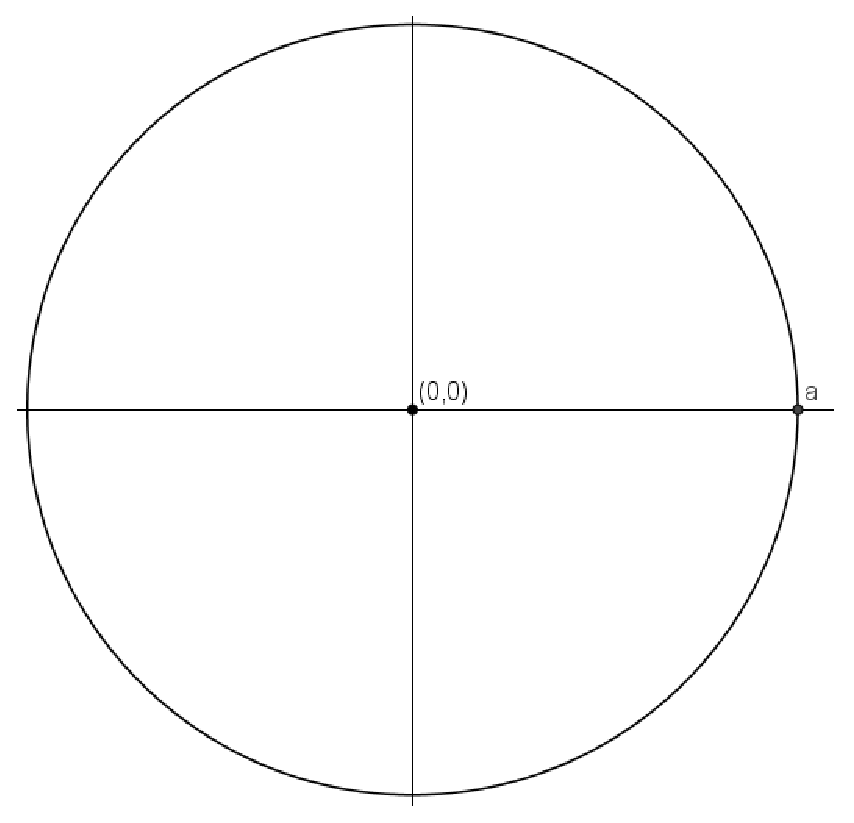
\includegraphics[width=0.2\linewidth]{\dir/Semana14-15/semana14-circulo} \ \ 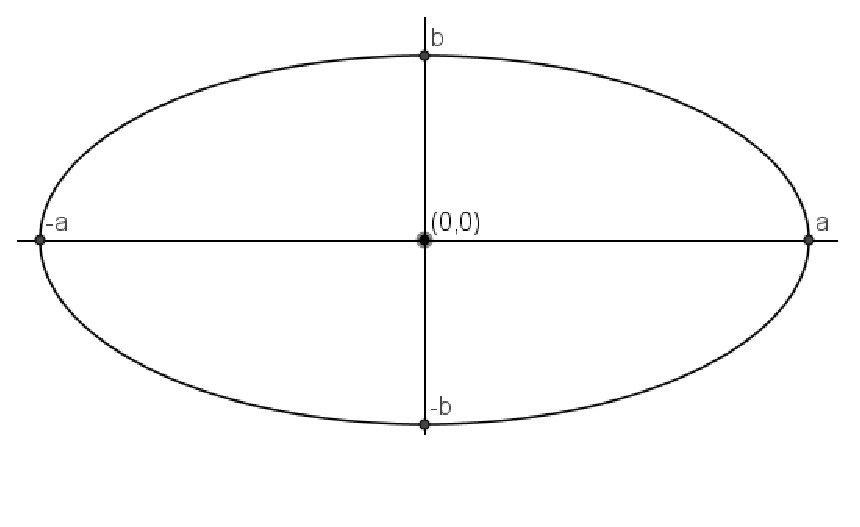
\includegraphics[width=0.3\linewidth]{\dir/Semana14-15/semana14-elipse} \ \ 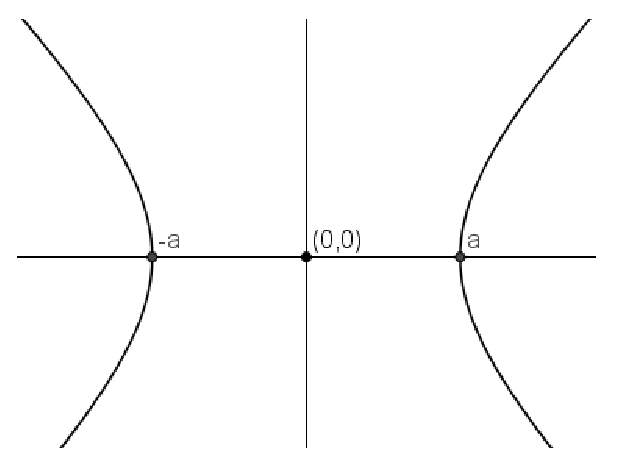
\includegraphics[width=0.3\linewidth]{\dir/Semana14-15/semana14-hiperbole}
	\end{center}
\end{figure}

\noindent Vamos ver como que a diagonalização de formas simétricas se aplica para conseguirmos identificar cônicas de formas quadráticas que possuem termos mistos.


\begin{example}
	Vamos identificar a cônica cuja equação é
	\[
	31 x_1^2 - 10\sqrt{3} x_1x_2 + 21 x_2^2 = 144.
	\] Podemos escrever
	\[
	\vec{x}^T A \vec{x} = 144, \quad \text{onde} \quad
	A = 
	\begin{bmatrix}
	31 & -5\sqrt{3} \\
	-5\sqrt{3} &  21
	\end{bmatrix}.
	\] Autovalores de $A$:
	\[
	p(\lambda) = (31 - \lambda)(21-\lambda) - 75 = 0 \implies \lambda^2 - 52 \lambda + 576
	= 0
	\]
	\[
	\implies \lambda = \frac{52 \pm \sqrt{2704 - 2304}}{2} = \frac{52 \pm 20}{2} = 26\pm 10 \implies \lambda_1 = 16, \ \lambda_2 = 36.
	\] Autovetores associados:
	\begin{itemize}
		\item  ao autovalor $\lambda_1 = 16$:
		\[
		\begin{bmatrix}
		15 & -5\sqrt{3} \\
		-5\sqrt{3} &  5
		\end{bmatrix} \sim
		\begin{bmatrix}
		3 & -\sqrt{3} \\
		0 &  0
		\end{bmatrix} \implies 
		3v_1 = \sqrt{3} v_2 \ \ \xrightarrow[\text{e já normalizando}]{\text{podemos escolher}} \ \  \vec{v}_1 = 
		\begin{bmatrix}
		1/2 \\ \sqrt{3}/2
		\end{bmatrix}.
		\]
		\item ao autovalor $\lambda_2 = 36$:
		\[
		\begin{bmatrix}
		-5 & -5\sqrt{3} \\
		-5\sqrt{3} &  -15
		\end{bmatrix} \sim
		\begin{bmatrix}
		1 & \sqrt{3} \\
		0 &  0
		\end{bmatrix} \implies 
		v_1 = - \sqrt{3} v_2 \ \ \xrightarrow[\text{e já normalizando}]{\text{podemos escolher}} \ \  \vec{v}_2 = 
		\begin{bmatrix}
		-\sqrt{3}/2 \\ 1/2
		\end{bmatrix}.
		\]
	\end{itemize} Temos
	\[
	P^{-1} A P = D =
	\begin{bmatrix}
	16 & 0 \\ 0 & 26
	\end{bmatrix}
	\] Assim, na base de $\bR^2$ determinada por $\{\vec{v}_1, \vec{v}_2\}$, podemos escrever a equação da equação cônica como
	\[
	\vec{x}^T A \vec{x} = \vec{y}^T D \vec{y} \implies 
	\begin{bmatrix}
	y_1 & y_2
	\end{bmatrix}
	\begin{bmatrix}
	16 & 0 \\ 0 & 26
	\end{bmatrix}
	\begin{bmatrix}
	y_1 \\ y_2
	\end{bmatrix} = 144.
	\] Isto pode ser reescrito como
	\[
	16 y_1^2 + 36 y_2^2 = 144 \ \leftrightsquigarrow \ \frac{y_1^2}{(144/16)} + \frac{y_1^2}{(144/36)} = 1 \ \leftrightsquigarrow \ \frac{y_1^2}{3^2} + \frac{y_1^2}{2^2} = 1.
	\] Esta equação é pode ser agora identificada como uma elipse nos ``novos eixos'' $\vec{v}_1$ e $\vec{v}_2$.
	\begin{center}
		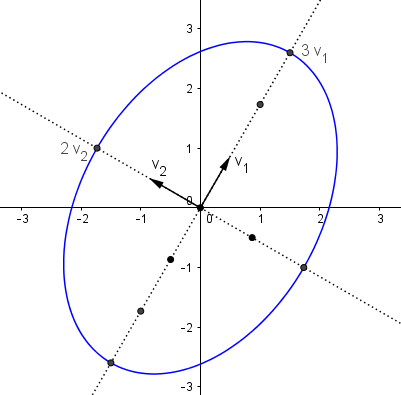
\includegraphics[width=0.5\linewidth]{\dir/Semana14-15/semana14-conicas2}
	\end{center}
	
	\noindent Observamos que quando a coordenada $y_1 = 0$ devemos ter que $y_2^2 = 2^2$, de modo que deve ser $\vec{x} = y_1 \vec{v}_1 + y_2 \vec{v}_2 = \pm 2 \vec{v}_2$, como na figura. Este é o análogo da análise que normalmente fazemos, só que agora na base ortonormal $\{\vec{v}_1, \vec{v}_2\}$
\end{example}


\section{Problemas de otimização restritos à esfera}

Nesta seção, estudamos alguns problemas de otimização bem específicos. Mais precisamente, podemos encontrar valores de máximo e mínimo de formas quadráticas
\[
Q(\vec{x}) = \vec{x}^T A \vec{x}
\] sujeitos à restrição 
\[
x_1^2 + x_2^2 + \cdots + x_n^2 = 1,
\] que caracteriza os pontos $(x_1, x_2, \dots, x_n) \in \bR^n$ que tem comprimento unitário, isto é, a esfera de raio 1 e centro na origem em $\bR^n$. Em outras palavras, nosso problema de otimização restrito consiste em achar, na esfera unitária, os vetores em que a forma quadrática $Q$ assume seu maior valor e seu menor valor.

Mais resumidamente, queremos:
\[
\text{maximizar/minimizar } Q(\vec{x}) \ \text{sujeito à restrição} \ \|\vec{x}\|=1.
\]

\noindent \textbf{Ideia por trás do método.} Sendo $A$ uma matriz simétrica, todos os seus autovalores são reais. Vamos ordená-los em forma crescente
\[
\lambda_1 \le \lambda_2 \le \cdots \le \lambda_n.
\] Podemos também encontrar uma base ortonormal de autovetores e, com eles, formar uma matriz ortogonal que diagonaliza $A$:
\[
P =  
\begin{bmatrix}
| & | &  & | \\
\vec{v}_1 & \vec{v}_2 & \cdots & \vec{v}_n \\
| & | &  & | \\
\end{bmatrix} \implies
P^{-1} A P = D = 
\begin{bmatrix}
\lambda_1 & 0  & \cdots & 0 \\
0 & \lambda_2  & \cdots & 0 \\
\vdots & \vdots & \ddots & \vdots \\
0 & 0 & \cdots & \lambda_n
\end{bmatrix}.
\] Nota que $P$, sendo ortogonal, preserva comprimentos (ver Observação \ref{sse} na seção seguinte). Assim, escrevendo $\vec{x} = P \vec{y}$, temos que $\|\vec{x}\| = 1$ se, e somente se, $\|\vec{y}\| = 1$. Além disso, esta matriz $P$ é a matriz ortogonal que diagonaliza $A$, de modo que, pelo que vimos na seção anterior,
\[
\vec{x}^T A \vec{x} = \vec{y}^T D \vec{y}.
\] Mas a forma quadrática $\vec{y}^T D \vec{y}$ é mais fácil de maximizar: sendo $\lambda_n$ a maior das entradas da diagonal principal de $D$, temos (já que cada $\lambda_j \le \lambda_n$ e $\|\vec{y}\| = 1$)
\[
\vec{y}^T D \vec{y} = \lambda_1 y_1^2 + \lambda_2 y_2^2 + \cdots + \lambda_n y_n^2 \le  \lambda_n (y_1^2 +y_2^2 + \cdots + y_n^2) = \lambda_n.
\] Logo, $\lambda_n$ é uma cota superior para $\vec{y}^T D \vec{y}$. Além disso, já que $D$ é uma matriz diagonal, esta cota superior é atingida pelo vetor $\vec{y} = \vec{e}_n$, o último vetor da base canônica de $\bR^n$. Traduzindo estas informações para a variável $\vec{x}$, temos que $\lambda_n$ é o valor máximo de $\vec{x}^T A \vec{x}$ (pois é igual a $\vec{y}^T D \vec{y}$) na esfera unitária. Além disso, este valor máximo é atingido quando $\vec{x} = P \vec{e}_n = \vec{v}_n$, um autovetor unitário associado com o maior autovalor $\lambda_n$.

\begin{exercise}
	Fazer toda a análise acima para o problema de minimização. \textit{Dica}: olhar para o menor autovalor.
\end{exercise}


\begin{example}\label{otimiz}
	Vamos maximizar a forma quadrática 
	\[
	Q(x_1, x_2, x_3) = 7 x_1^2 + x_2^2 + 7x_3^2 - 8 x_1x_2 - 4x_1x_3 - 8 x_2x_3,
	\] sujeito à restrição $x_1^2 + x_2^2 + x_3^2 = 1$.
	
	Note que podemos escrever
	\[
	\vec{x} = 
	\begin{bmatrix}
	x_1 \\ x_2 \\ x_3
	\end{bmatrix} \implies 
	Q(\vec{x}) = \vec{x}^T 
	\begin{bmatrix}
	7 & -4 & -2 \\
	-4 &  1 & -4 \\
	-2 & -4 &  7 \\
	\end{bmatrix}\vec{x}.
	\] Precisamos determinar o maior autovalor e um autovetor unitário associado. O polinômio característico de $A$ é dado por 
	\[
	\det 
	\begin{bmatrix}
	7 - \lambda & -4 & -2 \\
	-4 &  1 - \lambda & -4 \\
	-2 & -4 &  7 - \lambda \\
	\end{bmatrix} = - \lambda^3 + 15 \lambda^2 - 27 \lambda - 243,
	\] cujas raízes são $\lambda_1 = -3$ e $\lambda_2 = 9$. Portanto, o valor máximo que a forma quadrática $Q$ assume na esfera unitária é $9$.
	
	Além disso, sabemos que qualquer um autovetor unitário associado com o autovalor $\lambda_2 = 9$ assume este valor máximo. Resolvemos
	\[
	A - 9 I = 
	\begin{bmatrix}
	-2 & -4 & -2 \\
	-4 & -8 & -4 \\
	-2 & -4 &  -2 \\
	\end{bmatrix} \sim
	\begin{bmatrix}
	1 & 2 & 1 \\
	0 & 0 & 0 \\
	0 & 0 & 0 \\
	\end{bmatrix} \implies \vec{v} =
	\begin{bmatrix}
	-2v_2 - v_3 \\ v_2 \\ v_3
	\end{bmatrix}  = v_2
	\begin{bmatrix}
	-2 \\ 1 \\ 0
	\end{bmatrix} + v_3
	\begin{bmatrix}
	-1 \\ 0 \\ 1
	\end{bmatrix}.
	\] Um autovetor (unitário!) possível é
	\[
	\frac{1}{\sqrt{2}}
	\begin{bmatrix}
	-1 \\ 0 \\ 1
	\end{bmatrix} = 
	\begin{bmatrix}
	-1/\sqrt{2} \\ 0 \\ 1/\sqrt{2}
	\end{bmatrix}.
	\] Conferimos que 
	\[
	Q \left(\frac{1}{\sqrt{2}}, 0, \frac{1}{\sqrt{2}}\right) = \frac{7}{2} + 0 + \frac{7}{2} - 0 + \frac{4}{2} - 0 = 9. \ \lhd
	\]
\end{example}


\begin{remark}[Opcional]
	Em cursos de cálculo com várias variáveis, estudamos multiplicadores de Lagrange, uma ferramenta para estudar problemas de otimização com restrição. De uma maneira geral, queremos
	\[
	\text{minimizar } f(x_1, x_2, \cdots, x_n) \text{ com a restrição } g(x_1, x_2, \cdots, x_n) = 0.
	\] O método dos multiplicadores de Lagrange nos dá uma condição necessária: se um ponto é de máximo/mínimo com restrição, então existe uma constante $\lambda$ tal que, neste ponto,
	\[
	\vec{\nabla} f = \lambda \vec{\nabla} g.
	\] Esta constante $\lambda$ é conhecida como um \textbf{multiplicador de Lagrange}. Como mencionamos, esta é uma condição necessária, de modo que não garante que o ponto é de mínimo/máximo. Na prática, depois de encontrarmos os possíveis valores de $\vec{x}$ e de $\lambda$, podemos substituir na função para ver quais são os pontos de mínimo e quais são os de máximo.
	
	Vejamos como esta técnica se aplicaria no Exemplo \ref{otimiz} que já resolvemos acima. Vamos considerar $f(x_1,x_2,x_3) = Q(x_1,x_2,x_3)$ e $g(x_1,x_2,x_3) = x_1^2 + x_2^2 + x_3^2 - 1$ Se estivermos em um ponto de máximo, então existe a constante $\lambda$ como acima. Calculamos:
	\[
	\vec{\nabla} Q = \left( 14x_1 - 8x_2 - 4 x_3, 2x_2 - 8 x_1 - 8 x_3, 14x_3 - 4 x_1 - 8 x_2 \right) 
	\] e 
	\[
	\vec{\nabla} g = \left( 2 x_1, 2 x_2, 2 x_3 \right) .
	\] A condição $\vec{\nabla} Q = \lambda \vec{\nabla} g$ nos diz que devemos resolver
	\[
	\begin{array}{c}
	14 x_1 - 8x_2 - 4 x_3 = 2 \lambda x_1 \\
	-8x_1 + 2x_2  - 8 x_3 = 2 \lambda x_2 \\
	- 4x_1 - 8 x_2 +14x_3 = 2 \lambda x_3 \\
	\end{array} \xrightarrow[\text{em cada eq.}]{\text{Simplifica um $2$}}
	\begin{bmatrix}
	7 & -4 & -2 \\
	-4 & 1 & -4 \\
	-2 & -4 & 7 \\
	\end{bmatrix} 
	\begin{bmatrix}
	x_1 \\ x_2 \\ x_3
	\end{bmatrix} = \lambda
	\begin{bmatrix}
	x_1 \\ x_2 \\ x_3
	\end{bmatrix}.
	\] Chegamos, por outro caminho, à mesma conclusão: $\lambda$ deve ser um autovalor e $\vec{x}$ um autovetor (unitário, já que $g(x_1,x_2,x_3) = 0$) associado$. \ \lhd$
\end{remark}


\section{Matrizes simétricas e prova do Teorema Espectral}

Nesta seção vamos utilizar a notação $\langle \vec{u}, \vec{v} \rangle$ para o produto escalar, ao invés de $\vec{u} \cdot \vec{v}$, para enfatizar qual é o vetor $\vec{u}$ e qual é o vetor $\vec{v}$ (em especial quando um deles está sendo multiplicado por uma matriz).

%Vejamos mais uma maneira equivalente de se dizer que uma matriz é simétrica.
\begin{remark}\label{sse}
	Uma matriz quadrada $A$, não necessariamente simétrica, cujos coeficientes são reais, satisfaz
	\[
	\langle A \vec{x}, \vec{y} \rangle = \langle\vec{x}, A^T \vec{y}\rangle, \quad \text{ para todos } \vec{x}, \vec{y} \in \bR^n.
	\] Isto se pode verificar ao analisar os coeficientes de $A \vec{x}$ e de $A^T \vec{y}$. Assim, uma matriz $A$ de ordem $n \times n$ é \textbf{simétrica} se, e somente se, satisfaz
	\[
	\langle A \vec{x}, \vec{y} \rangle = \langle\vec{x}, A \vec{y}\rangle, \quad \text{ para todos } \vec{x}, \vec{y} \in \bR^n.
	\]
	Outras formas de escrever esta mesma coisa (concorda?) são
	\[
	A \vec{x} \cdot \vec{y} = \vec{x} \cdot A \vec{y}, \quad \text{ para todos } \vec{x}, \vec{y} \in \bR^n
	\] e 
	\[
	\vec{y}^T A \vec{x} = \vec{x}^T A \vec{y}, \quad \text{ para todos } \vec{x}, \vec{y} \in \bR^n.
	\]
\end{remark}

\begin{remark}
	A observação anterior nos permite estender a definição de matriz simétrica para transformações lineares, pois é independente do sistema de coordenadas utilizado (depende apenas de uma escolha de produto interno/escalar). 
\end{remark}

A equivalência que foi apresentada na Observação \ref{sse} é muito útil na análise de matrizes simétricas. Vamos ver como se aplica diversas vezes na demonstração do Teorema Espectral que será dividida em três proposições preliminares. Cada uma delas apresenta, em ordem, o procedimento usual que viemos utilizando para diagonalizar matrizes: análise dos autovalores, construção dos autoespaços e verificação de que é possível formar uma base de autovetores. Neste caso de uma matriz simétrica, veremos que, além de tudo, é possível encontrar uma base ortonormal de autovetores.

\begin{proposition}\label{reais}
	Os autovalores de uma matriz simétrica $A$, de entradas reais, são números reais.
\end{proposition}

\begin{proof}
	Seja $\lambda$ uma raiz do polinômio característico de $A$, que pode ser um número real ou um número complexo. Podemos encontrar um vetor $\vec{v}$, de entradas possivelmente complexas, tal que $A\vec{v} = \lambda \vec{v}$. A menos de um passo de normalização, podemos pensar que $\|\vec{v}\| = 1$. Vamos verificar que de fato $\lambda$ é um número real. Para isto, vamos mostrar que $\lambda$ é igual ao seu conjugado, $\lambda = \bar{\lambda}$, de forma que a parte imaginária de $\lambda$ deve ser igual a zero. Sendo $A$ simétrica, temos que
	\[
	\overline{\lambda} = \overline{\lambda \|\vec{v}\|^2} = \overline{\langle \lambda \vec{v}, \vec{v} \rangle} = \overline{\langle A \vec{v}, \vec{v} \rangle} = \overline{\langle \vec{v}, A \vec{v} \rangle} = \overline{\langle \vec{v}, \lambda \vec{v} \rangle} = \lambda \overline{\langle \vec{v}, \vec{v} \rangle} = \lambda.
	\] A simetria de $A$ foi necessária (apenas) no quarto sinal de igualdade acima. Ainda, na penúltima igualdade, utilizamos sem muitos comentários uma propriedade do produto interno em espaços vetoriais com escalares complexos, a saber, que
	\[
	\langle\vec{u}, \vec{v}\rangle \stackrel{\text{def}}{=} \sum_{i=1}^{n} u_i \overline{v}_i.
	\] Os conjugados das componentes do segundo vetor aparecem para que a fórmula usual para o comprimento continue sendo válida:
	\[
	\| \vec{u} \|^2 = \langle\vec{u}, \vec{u}\rangle = \sum_{i=1}^{n} u_i \overline{u}_i = \sum_{i=1}^{n} |u_i|^2.
	\] Desta forma, continua valendo que
	\[
	\langle k\vec{u}, \vec{v} \rangle = k \langle \vec{u}, \vec{v}\rangle, \quad \text{enquanto que} \quad \langle \vec{u},k\vec{v}\rangle = \overline{k} \langle \vec{u}, \vec{v}\rangle. \qedhere
	\]
\end{proof}

\begin{proposition}\label{ortog}
	Se $A$ é uma matriz simétrica, então autovetores associados a autovalores distintos são ortogonais.
\end{proposition}

\begin{proof}
	Sejam $\lambda_1$ e  $\lambda_2$ autovalores distintos de $A$ e $\vec{v}_1, \vec{v}_2$ respectivos autovetores. Então (observe que é necessário que $A$ seja simétrica na segunda e na última igualdade!)
	\[
	\lambda_1 \langle \vec{v}_1, \vec{v}_2\rangle = \langle \lambda_1 \vec{v}_1, \vec{v}_2\rangle = \langle A \vec{v}_1, \vec{v}_2\rangle = \langle \vec{v}_1, A \vec{v}_2\rangle = \overline{\lambda}_2 \langle \vec{v}_1, \vec{v}_2\rangle = \lambda_2 \langle \vec{v}_1, \vec{v}_2\rangle,
	\] de modo que $(\lambda_1 - \lambda_2)\langle \vec{v}_1, \vec{v}_2\rangle = 0$. Já que estamos supondo que os autovalores são distintos, $\lambda_1 \neq \lambda_2$, concluimos que $\langle \vec{v}_1, \vec{v}_2\rangle = 0$.
\end{proof}


\begin{proposition}\label{dimens}
	Seja $A$ uma matriz simétrica. Então, a dimensão do autoespaço associado a um autovalor é igual à multiplicidade deste autovalor.
\end{proposition}

\begin{proof}
	Suponhamos que $\lambda_1$ é um autovalor de $A$ de multiplicidade $k$. Seja $\vec{v}_1$ um autovetor unitário associado. Podemos encontrar uma base ortonormal de $\bR^n$ da qual $\vec{v}_1$ faz parte, isto é, podemos encontrar vetores unitários $\vec{y}_j$ de modo que
	\[
	\{ \vec{v}_1, \vec{y}_2, \vec{y}_3, \dots, \vec{y}_n \}
	\] é uma base ortonormal de $\bR^n$.
	
	Considere a matriz $Q$ cujas colunas são os elementos desta base:
	\[
	Q = 
	\begin{bmatrix}
	| & | & | & & | \\
	\vec{v}_1 & \vec{y}_2 & \vec{y}_3 & \cdots &  \vec{y}_n \\
	| & | & | & & | \\
	\end{bmatrix},
	\] que é, consequentemente, ortogonal. Vamos calcular $Q^{-1} A Q = Q^T A Q$. O produto $AQ$ pode ser interpretado como o produto de $A$ por cada uma das colunas de $Q$:
	\[
	AQ = 
	\begin{bmatrix}
	| & | & | & & | \\
	A \vec{v}_1 & A \vec{y}_2 & A \vec{y}_3 & \cdots &  A\vec{y}_n \\
	| & | & | & & | \\
	\end{bmatrix} = 
	\begin{bmatrix}
	| & | & | & & | \\
	\lambda_1 \vec{v}_1 & A \vec{y}_2 & A \vec{y}_3 & \cdots &  A\vec{y}_n \\
	| & | & | & & | \\
	\end{bmatrix}.
	\] Logo,
	\[
	Q^TAQ =
	\begin{bmatrix}
	\text{---} & \vec{v}_1 & \text{---} \\
	\text{---} & \vec{y}_2 & \text{---} \\
	\text{---} & \vec{y}_3 &\text{---} \\
	& \vdots    &     \\
	\text{---} & \vec{y}_n & \text{---} \\      
	\end{bmatrix}
	\begin{bmatrix}
	| & | & | & & | \\
	\lambda_1 \vec{v}_1 & A \vec{y}_2 & A \vec{y}_3 & \cdots &  A\vec{y}_n \\
	| & | & | & & | \\
	\end{bmatrix}
	\]
	\[
	\implies Q^TAQ =
	\begin{bmatrix}
	\lambda_1\langle \vec{v}_1, \vec{v}_1 \rangle & \langle \vec{v}_1, A\vec{y}_2 \rangle & \langle \vec{v}_1, A\vec{y}_3 \rangle & \cdots & \langle \vec{v}_1, A\vec{y}_n \rangle \\
	\lambda_1\langle \vec{y}_2, \vec{v}_1 \rangle & \langle \vec{y}_2, A\vec{y}_2 \rangle & \langle \vec{y}_2, A\vec{y}_3 \rangle & \cdots & \langle \vec{y}_2, A\vec{y}_n \rangle \\
	\lambda_1\langle \vec{y}_3, \vec{v}_1 \rangle & \langle \vec{y}_3, A\vec{y}_2 \rangle & \langle \vec{y}_3, A\vec{y}_3 \rangle & \cdots & \langle \vec{y}_3, A\vec{y}_n \rangle \\
	\vdots & \vdots & \vdots & \ddots & \vdots \\
	\lambda_1\langle \vec{y}_n, \vec{v}_1 \rangle & \langle \vec{y}_n, A\vec{y}_2 \rangle & \langle \vec{y}_n, A\vec{y}_3 \rangle & \cdots & \langle \vec{y}_n, A\vec{y}_n \rangle \\
	\end{bmatrix}
	\] Observamos que, pela simetria de $A$ e por ser $	\{ \vec{v}_1, \vec{y}_2, \vec{y}_3, \dots, \vec{y}_n \}$ um conjunto ortonormal, temos 
	\[
	\langle \vec{v}_1, A\vec{y}_j \rangle = \langle A\vec{v}_1, \vec{y}_j \rangle = \lambda_1 \langle \vec{v}_1, \vec{y}_j \rangle = 0, \quad \text{para qualquer índice } j.
	\]Logo,
	\[
	\implies Q^TAQ =
	\begin{bmatrix}
	\lambda_1 & 0 & 0 & \cdots & 0 \\
	0 & b_{22} & b_{23} & \cdots & b_{2n} \\
	0 & b_{32} & b_{33} & \cdots & b_{3n} \\
	\vdots & \vdots & \vdots & \ddots & \vdots \\
	0 & b_{n2} & b_{n3} & \cdots & b_{nn} \\
	\end{bmatrix} \stackrel{\text{def}}{=} \hat{A}.
	\] Chamamos os coeficientes restantes de $b_{ij}$ simplesmente porque não nos interessa muito quanto valem (notamos, no entanto, que a simetria de $A$ implica que $b_{ij} = b_{ji}$). Observamos que 
	\[
	\det \left( A - \lambda I \right) = \det \left( Q^{-1} (A - \lambda I) Q \right) =	\det \left( \hat{A} - \lambda I \right) = (\lambda_1 - \lambda) \cdot \det (B - \lambda I),
	\] onde $B$ é a matriz de ordem $(n-1)\times (n-1)$ dada por $(b_{ij})$. Além disso, se a multiplicidade de $\lambda_1$ como autovalor de $A$ for maior do que $1$, devemos ter, pela igualdade acima, que $\lambda_1$ também é um autovalor de $B$. Desta forma, $\hat{A}$ possui um autovetor unitário $\vec{v}_2$ associado com $\lambda_1$ que está contido em $\Span \{ \vec{y}_2, \vec{y}_3, \dots, \vec{y}_n \}$ e, portanto, é distinto e linearmente independente a $\vec{v}_1$. O processo de Gram-Schmidt permite obter $\{\vec{v}_1, \vec{v}_2\}$ ortonormais.
	
	A partir daí, repetimos o processo completando o conjunto $\{\vec{v}_1, \vec{v}_2\}$ a uma base ortonormal $\{ \vec{v}_1, \vec{v}_2, \vec{y}_3, \dots, \vec{y}_n \}$ de $\bR^n$. Daí vamos obter um terceiro autovetor ortogonal aos anteriores e unitário. Procedemos desta meneira até encontrar $k$ autovetores ortogonais e unitários associados ao autovalor $\lambda_1$. Assim, o autoespaço $\Nul (A - \lambda_1 I)$ tem dimensão $k$, que é igual à multiplicidade do autovalor $\lambda_1$.
\end{proof}

\subsection{Prova do Teorema Espectral}

O Teorema Fundamental da Álgebra afirma que todo polinômio não constante de grau $n$ possui exatamente $n$ raízes complexas. Sendo assim, qualquer matriz $A$ de ordem $n\times n$ possui $n$ autovalores complexos. No entanto, sendo $A$ uma matriz simétrica, a Proposição \ref{reais} garante que todas estes $n$ autovalores são todos reais. Vamos denotar por
\[
\lambda_1, \lambda_2, \dots, \lambda_k \in \bR
\] os autovalores distintos de $A$ e por $m_1, m_2, \dots, m_k$ suas respectivas multiplicidades. Temos, em particular, que $m_1 + m_2 + \cdots + m_k = n$.

Pela Proposição \ref{dimens}, a dimensão do autoespaço associado a $\lambda_1$ é $m_1$. Podemos encontrar (da maneira usual, por escalonamento) uma base de autovetores
\[
\Nul (A - \lambda_1 I) = \Span \{ \vec{u}_1, \vec{u}_2, \dots, \vec{u}_{m_1} \}.
\] Estes autovetores, possivelmente não são ortogonais, mas, aplicando o Processo de Gram-Schmidt, podemo obter uma base ortonormal de $\Nul (A - \lambda_1 I)$:
\[
\Nul (A - \lambda_1 I) = \Span \{ \vec{v}_1, \vec{v}_2, \dots, \vec{v}_{m_1} \}.
\] Fazendo este mesmo procedimento para cada um dos autovalores, obtemos $n$ autovetores, que, consequentemente, formam uma base para $\bR^n$. Logo, $A$ é diagonalizável.

Além disso, a Proposição \ref{ortog} garante que todo autovetor de um autoespaço é ortogonal a todo autovetor de outro autoespaço (associado a um autovalor diferente). Temos então $k$ autoespaços, cujas bases são ortonormais e elementos da base de um autoespaço são ortogonais aos elementos das outras bases. Segue daí que a união das bases dos autoespaços, como consideramos, é uma base \textit{ortonormal} para $\bR^n$.

Explicitamente, a matriz
\[
P = 
\begin{bmatrix}
| & | & & | \\
\vec{v}_1 & \vec{v}_2 & \cdots &  \vec{v}_n \\
| & | &  & | \\
\end{bmatrix}
\] formada pelos autovetores é ortogonal e 
\[
P^{-1} A P = D = 
\begin{bmatrix}
\lambda_1 & 0 & 0 & \cdots & 0 \\ 
0 & \lambda_2 & 0 & \cdots & 0 \\ 
0 & 0 & \lambda_3 & \cdots & 0 \\ 
\vdots & \vdots & \vdots & \ddots & \vdots \\ 
0 & 0 & 0 & \cdots & \lambda_n \\ 
\end{bmatrix}.
\] Sendo $P$ ortogonal, tem-se ainda que $P^{-1} = P^T$.


\end{document} 